\documentclass[12pt]{scrartcl}
\usepackage{graphicx}
\usepackage{pdfpages}

\begin{document}

\begin{titlepage}
\begin{center}

\vspace*{3.0 cm}
{\Huge Public Static Void Main}\\[0.7cm]
{\Large Requirements Document, Version 1}\\[3.8cm]
{\Large \today}\\[0.5cm]
Adam Schwalm\\
Eli Hunnicutt\\
Andrew LaFrance\\
Tyler Bertrand\\
Martin Kinsey\\[4.0cm]

Group Number: 5\\
Lab Instructor: Ajay Bandi
  

  
\end{center}
\end{titlepage}


\newpage\null\thispagestyle{empty}\newpage

\tableofcontents

\newpage\null\thispagestyle{empty}\newpage

\section{Overview Module Diagram}
\includegraphics[scale=0.9]{dependency.pdf}

\section{Detailed Class Diagrams}
\subsection{Data Modules}
\subsubsection{Category}
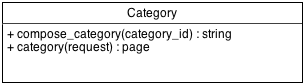
\includegraphics[keepaspectratio]{umls/category_uml.png}
\begin{description}
\item [compose\_category(category\_id)] Get the threads in a category as formatted HTML
\item [category(request)] Handle the GET request for the category.html page
\end{description}

\subsubsection{Database}
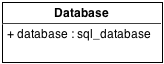
\includegraphics[keepaspectratio]{umls/database_uml.png}
\begin{description}
\item [database] Member which allows execution of database queries 
\end{description}

\subsubsection{Execute}
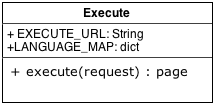
\includegraphics[keepaspectratio]{umls/execute_uml.png}
\begin{description}
\item [EXECUTE\_URL] Constant value which is the url code execution is sent to for completion
\item [LANGUAGE\_MAP] Constant which maps the names of languages used by the markup to the strings required by the EXECUTE\_URL
\item[execute(request)] Handles GET to the execute/ URL. The function queries the EXECUTE\_URL API with a json object and returns an unformatted string as the result
\end{description}

\subsubsection{Login}
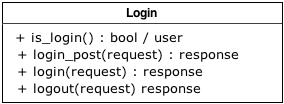
\includegraphics[keepaspectratio]{umls/login_uml.png}
\begin{description}
\item [is\_login()] Returns False if the user is not logged in, otherwise it returns a named\_tuple with the username, user\_id and permissions
\item [login\_post(request)] Handles POST requests to /login. Returns a redirect  and cookie
\item [login(request)] Handles GET requests to /login.html. Renders the page.
\item [logout(request)] Handles POST to /logout.html. Gives the user a cookie which has already expired to force the browser to remove them, logging out the user.
\end{description}

\subsubsection{Mail}
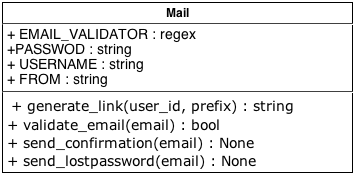
\includegraphics[keepaspectratio]{umls/mail_uml.png}
\begin{description}
\item [EMAIL\_VALIDATOR] Compiled regular expression used to determine whether an email is possibly valid
\item [PASSWORD] Stores password used to login to gmail server used by the forum
\item [USERNAME] Stores the username of the gmail account used by the forum
\item [FROM] Constant address email address used by the forum to send email
\item [generate\_link(user\_id, prefix, link\_dict)] Generate a one-time expiring link of 100 random hex digits (generated by applying SHA-512 to 100 random bits)
\item [validate\_email(email)] Returns True if the ‘email’ matches the “EMAIL\_VALIDATOR” regex
\item [send\_confirmation(email)] Sends an email to the given address containing a one-time link to validate the account
\item [send\_lostpassword(email)] Send an email to the email with a link to re-enter the password
\end{description}

\subsubsection{Markup}
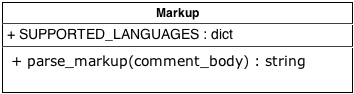
\includegraphics[keepaspectratio]{umls/markup_uml.png}
\begin{description}
\item [parse\_markup(comment\_body)] Parse a comment for the markup language, adding the necessary HTML and SQL entries
\item [SUPPORTED\_LANGUAGES] List of languages supported by the syntax highlighter.
\end{description}

\subsubsection{Message}
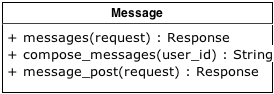
\includegraphics[keepaspectratio]{umls/message_uml.png}
\begin{description}
\item [messages(request)] Generate messages.html for a logged-in user. 404’s if user is not logged in.
\item [compose\_messages(user\_id)] Generate the HTML for the posts / query the database for the body of messages
\item [ message\_post(request)] Handles POST request to send a message
\end{description}

\subsubsection{Post}
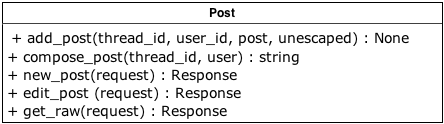
\includegraphics[keepaspectratio]{umls/post_uml.png}
\begin{description}
\item [add\_post(thread\_id, user\_id, post, unescaped)] Add post to the database with the given information
\item [compose\_posts(thread\_id, user)] Compose the HTML of the posts and return it as a string
\item [new\_post(request)] Handles POST request to add a new post
\item [edit\_post(request)] Handles POST request to edit a post
\item [get\_raw(request)] Return the unescaped content of a post (for editing purposes)
\end{description}

\subsubsection{Register}
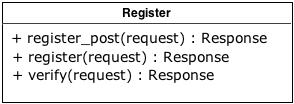
\includegraphics[keepaspectratio]{umls/register_uml.png}
\begin{description}
\item[register\_post(request)] Handles POST request to register a new user. Dispatches an email to verify that the user controls the email account
\item [register(request)] Handles GET request to register.html, composes page
\item [verify(request)] Handles GET to /verify/ which activates a users account
\end{description}

\subsubsection{Request}
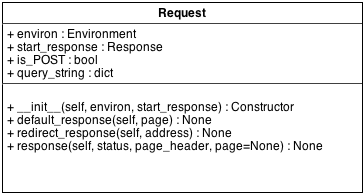
\includegraphics[keepaspectratio]{umls/request_uml.png}
\begin{description}
\item [\_\_init\_\_(self, environ, start\_response)] Constructor, parses the query string and determines type of request
\item [default\_response(self, page)] Generates a page with 200 OK response
\item [ redirect\_response(self, address)] Generates a 301 REDIRECT response to address
\item [reponse(self, status, page\_header, page=None)] Generate a page with status as the response status, page as the content and page\_header as the header
\end{description}


\subsubsection{Reset}
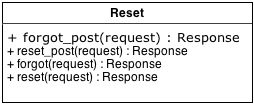
\includegraphics[keepaspectratio]{umls/reset_uml.png}
\begin{description}
\item [forgot\_post(request)] Sends a reset password link to specified email, if there is a user account with that address.
\item [reset\_post(request)] When given a valid reset key, directs the user to enter and verify a new password. If the passwords match, stores an encrypted version of the password into the database then deletes the reset key from the list of valid keys. Then directs the user to login with the new password.
\item [forgot(request)] Generates the page that prompts user to enter their email address for a forgotten password.
\item [reset(request)] Generates the page for resetting a user’s password.
\end{description}

\subsubsection{Search}
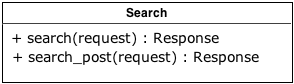
\includegraphics[keepaspectratio]{umls/search_uml.png}
\begin{description}
\item [search(request)] Handles GET request to post.html, does a database query to determine the contents
\item [search\_post(request)] Handles POST to search, returns a redirect to the search page
\end{description}

\subsubsection{Settings}
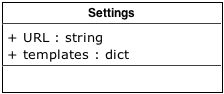
\includegraphics[keepaspectratio]{umls/settings_uml.png}
\begin{description}
\item [URL] Stores an internal URL
\item [templates] Replaces dynamic content tags with the specified content
\end{description}

\subsubsection{Thread}
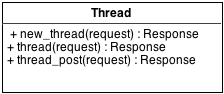
\includegraphics[keepaspectratio]{umls/thread_uml.png}
\begin{description}
\item [new\_thread(request)] Presents the user with the new thread page, allowing them to create a thread under a chosen category
\item [thread(request)] Generates a thread’s page, given the thread\_id number. If the thread does not exist, returns a 404 error
\item [thread\_post(request)] Allows the user to create a new post on a thread, prompts to login if the user is not
\end{description}

\subsubsection{User}
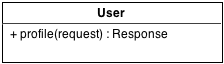
\includegraphics[keepaspectratio]{umls/user_uml.png}
\begin{description}
\item [profile(request)] Generates the user’s profile page, or returns 404 if the user does not exist
\end{description}

\section{Sequence Diagrams}
\subsection{Search}
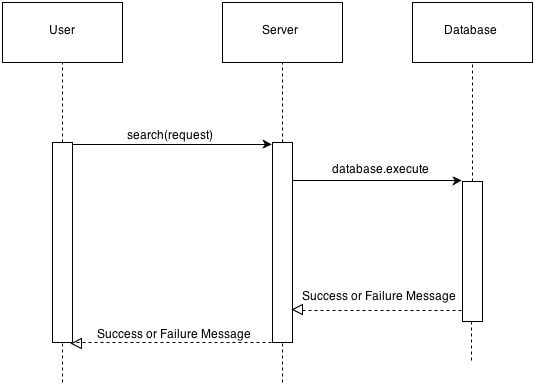
\includegraphics[keepaspectratio, scale=0.85]{sequence/search.png}

\subsection{Reset Password}
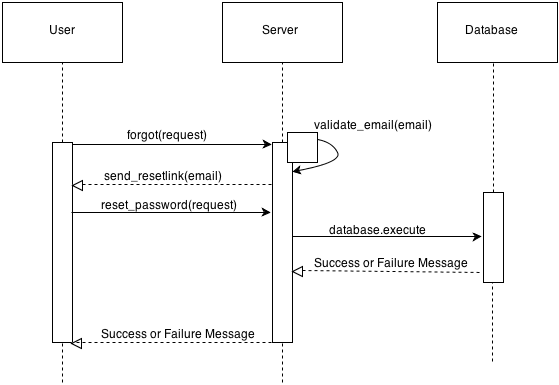
\includegraphics[keepaspectratio, scale=0.85]{sequence/reset.png}

\subsection{Create Thread}
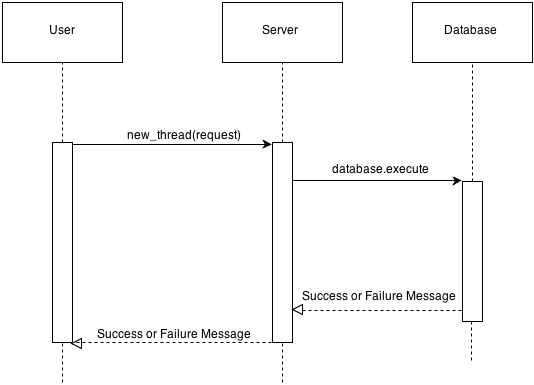
\includegraphics[keepaspectratio, scale=0.85]{sequence/createthread.png}

\subsection{Edit Post}
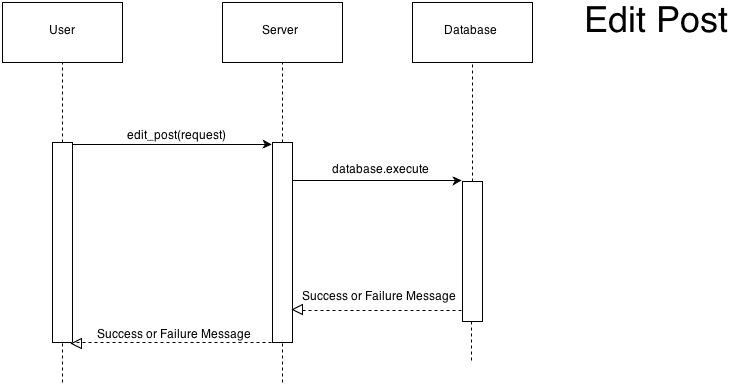
\includegraphics[keepaspectratio, scale=0.9]{sequence/editpost.png}

\newpage

\section{Appendix A - Database Design}

\textbf{users} \hfill \textbf{comments}\\*
*user\_id \hfill *comment\_id\\*
username \hfill \#thread\_id\\*
pass\_hash \hfill body\\*
email \hfill raw\\*
admin \hfill timestamp\\*
verified \hfill \#user\_id\\*
timestamp \\*
\\*
\textbf{categories} \hfill \textbf{code\_samples}\\*
*category\_id \hfill *sample\_id\\*
name \hfill language\\*
\hfill raw\\*
\hfill body\\*

\textbf{threads} \hfill \textbf{messages}\\*
*thread\_id \hfill *message\_id\\*
\#category\_id \hfill body\\*
title \hfill \#from\_id\\*
\#op\_id \hfill \#to\_id\\*
timestamp \hfill timestamp\\*

\section{Appendix B - Tasks and Assignments}
\begin{description}
\item [Requirements Presentation] - Martin Kinsey
\item [Design Presentation] - Adam Schwalm, Andrew LaFrance
\item [Final Presentation] - Tyler Bertrand, Eli Hunnicutt
\vspace{4mm}
\item [Adam Schwalm] - Backend Design, Server work
\item [Eli Hunnicutt] - Javascript Management, Design
\item [Andrew LaFrance, Martin Kinsey] - Graphic Design, Frontend Design work
\item [Tyler Bertrand] - Database Design, Management
\end{description}

\end{document}
